\documentclass{report}

\usepackage[utf8]{inputenc} % un package
\usepackage[T1]{fontenc}      % un second package
\usepackage[francais]{babel}  % un troisième package
\usepackage{graphicx}       %un quatrième package
\graphicspath{ {C:/Users/alexandre/Documents/Cours/ESIEE/E3T/S1/P2/IGI-3006/} }

\title{Rapport de projet - IGE-3006}
\author{Alexandre \bsc{Causse} - Jérémy \bsc{Fornarino}}
\date{Année scolaire : 2016-2017}

\begin{document}

\maketitle

\renewcommand{\contentsname}{Sommaire} 
\tableofcontents
\listoffigures
\newpage

\chapter*{Introduction}
Le gomoku est un jeu de plateau consistant à aligner n pions sur les intersection d'un plateau de jeu de taille n*n.
Le but de ce projet est de créer un plateau de jeu pour le Gomoku et une intelligence artificielle capable d'évaluer l'efficacité de chaque coup afin de maximiser les chances de victoire.


\part{Rapport technique}
	\chapter{Présentation des choix technologiques}
		\section{Technologie utilisée}
		% Utilisation de Java, et de JavaFX pour l'ihm
Nous avons choisi comme langage de programmation Java car celui-ci nous semblait le plus adapté pour créer les différentes parties constituant le jeu.De plus ce langage nous permet, pour l'implémentation de l'interface homme machine, de nous servir de JavaFX et ainsi d'obtenir des rendus de bonne qualité et donc une meilleure expérience de jeu pour l'utilisateur.
		\section{Organisation du code}
		% --> Là on calle le diagramme de classe final en intro	
		%insérer diagramme de classes
            Dans cette partie nous allons exposer les différentes classes mises en jeu dans notre projet afin de comprendre l'architecture globale. Cette architecture est représentée à l'aide du diagramme de classe (cf : figure \ref{DDC}).
            Nous avons mis en place trois différents packages qui nous permettent d'organiser nos classes en fonction de leur utilité.
            \begin{figure}[!t]
            	\centering
                \caption{DDC, Diagramme de classes}
                \label{DDC}
                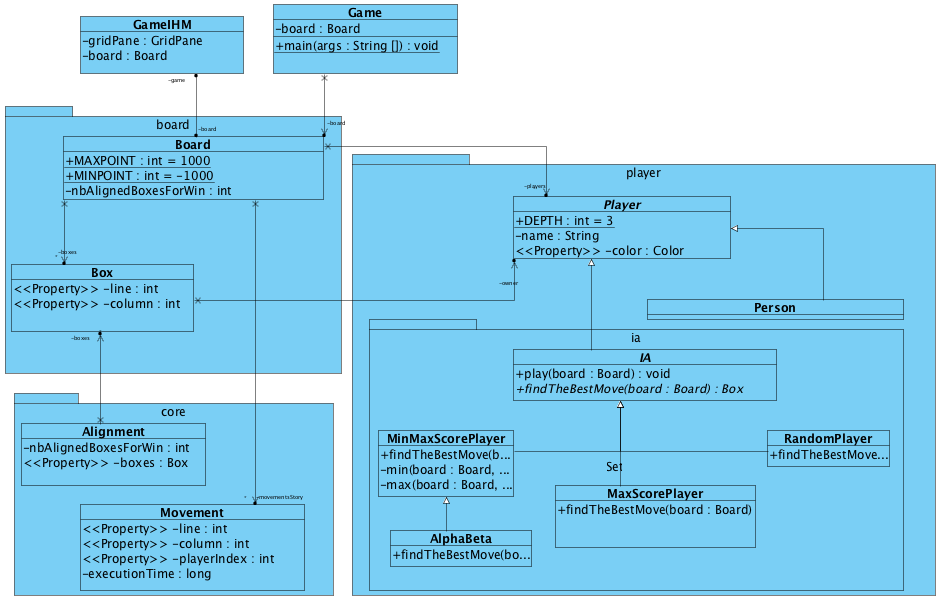
\includegraphics[scale=0.50]{diagrammeDeClasses.png}
            \end{figure}
			
			\subsection{Le package board}\label{packageBoard}
               		\paragraph{}
                			Le package \textit{board} est l'essence du jeux. En effet il contient la classe du même nom, \textit{Board}, ainsi que la classe \textit{Box}.
                		\paragraph{La classe board}\label{classeBoard}
               			 Cette classe représente le plateau de jeux. Elle contient un tableau avec l'ensemble des cases (cf : \ref{classBox}), les deux joueurs et le nombre de pions qu'il faut aligner pour gagner.
               			 De plus elle contient toutes les méthodes permettant l'évaluation du plateau de jeu à l'état courant. Par exemple les méthodes isFinished() et getNumberOfMove() permettent respectivement de
               			 déterminer une victoire et le nombre de coups déjà joués. Le nombre de coups déjà joués peut être calculé car nous avons mis en place un historique des mouvements effectués
               			 par l'intermédiaire d'un tableau de "Movement" (cf : \ref{pckCore}).
               			 Par ailleurs cet historique nous permet d'annuler le dernier coup jusqu'à atteindre la "racine" de l'arbre de jeu.

                    \paragraph{La classe box} \label{classBox}

               Cette classe permet de contenir l'emplacement de la case sur le tableau.
               La classe box permet également savoir si une case est prise par un joueur (cf : \ref{pckPlayer}) ou non.

			\subsection{Le package player} \label{pckPlayer}
			Ce package contient toutes les classes permettant de donner la main à un "joueur" celui-ci pouvant être un humain ou une intelligence artificielle.

			\paragraph{La classe Player}
			C'est une classe abstraite qui va permettre de définir la structure de base pour les différents types de joueurs.
			  Elle définit une méthode play(Board board) abstraite qui est utilisée par la board pour jouer.
            \subsubsection{Le package ia}
              Ce package contient l'ensemble des intelligences artificielles. L'ensemble des classes représentant une intelligence artificielle heritent de la classe abstraite IA.
              \paragraph{La classe abstraite IA}
              Cette classe hérite de la classe Player, elle définit le corps de la méthode play(Board board) ainsi qu'une méthode abstraite \textit{findTheBestMove(Board board)}.
              Cette methode demande aux filles de IA le meilleur coup à effectuer pour que l'IA le joue elle-même.

			\subsection{Le package core}\label{pckCore}
			Il contient deux classes qui permettent d'ordoner des informations afin de s'en servir par la suite.

			\subsection{Le package principal}
			Dans le "package principal", nous pouvons observer qu'il existe deux classes qui sont en dehors de tout package (Game et GameIHM).
			Ces classes nous permettent l'execution du jeux dans deux version differentes.
			La première version \textit{GameIHM} nous permet de proposer une interface graphique à nos utilisateurs.
			La seconde version \textit{Game} nous a permis de réaliser des test (cf : \ref{fichierCSV}) et d'executer le script sans
			interface homme machine (IHM) d'où l'importance de rendre le plateau de jeu totalement indépendant.
			% --> Là on explique la classe Board, on passe très rapidement sur Game

			% --> Explication de la classe box
			% --> Explication de la classe Player et de la classe IA
			% % --> Pour les players il faut dire qu'elle definit une methode play, ce qui nous permet de ne pas avoir à la gerer ensuite d'un joueur à l'uatre, c'est rien d'autre que la structure et les methodes de bases
			% % --> La classe IA definit une structure predefinit pour l'ensemble des IA qu'on voudra mettre en place avec l'ajout de la methode "findTheBestMove", ce qui nous permet d'avoir différents algo possible dans notre programme et donc de pouvoir tester d'un algo à un autre
	        %---> alignment et movement
	\chapter{Description des algorithmes}
	%% ATTENTION : Bien parler de la pronfondeur, et expliquer que plus on va taper dans le fond plus l'algo est precis et a de chance de gagner, et moins il est rapide.
	Dans cette partie nous allons vous expliquer les différents algorithmes que nous avons décidé d'implémenter et d'utiliser dans notre projet.
		\section{Random}
		% --> Là on explique que pour commencer on a créer une IA Random, ca nous a permit de mettre en place la structure de notre code et de tester les différentes methodes relatives a la board en mettant de côté la phase algorithmiques qui viendra plus tard
		Cet algorithme va jouer de façon autonome sur n'importe quelle case libre du jeu de façon aléatoire. Il n'est pas très efficace car il ne prend pas en compte les coups joués par l'adversaire et ses chances de victoires sont assez faibles. Ainsi nous avons pensé à une première une première évolution qu'est le max score.
		\section{Max score}
		% Dans cette section nous expliquerons que on a commencé par créer un algorithme "max", cette alogrithmes permet de connaitre le coup qui nous rapportera le plus de point. On va expliquer comment il fonctionne (#schéma)
		% On concluera sur le fait que même si on a plus de chance de gagner grâce à cet algo, il pose des problèmes du fait qu'il ne prévoit pas que l'adversaire puisse gagner donc il ne lui bloquera pas ses coups
		% --> Transition en douceur vers l'algorithme MinMax
		Cet algorithme est la première étape permettant d'augmenter les chances de victoires. Le principe est qu'il cherche le meilleur coup (le "Max") à jouer pour gagner, celui qui rapportera le plus de points. Ainsi avec cette méthode les chances de victoires sont accrues cependant on peut lui reprocher de ne toujours pas prendre en compte les placements de pions de l'autre joueur et c'est cette dernière amélioration qui sera apportée dans l'algorithme suivant.
		\section{Min Max}
		 \begin{figure}[!b]
             	    \caption{Schéma min-max (source : Wikipedia)}
             	    \label{minmaxWikipedia}
             	    \includegraphics[scale=0.60]{Min_Max_Sample_3.png}
             	\end{figure}
		% Description de l'algorithme, explication de son fonctionement, l'avantage avec celui là
		% On concluera sur le fait que beaucoup de coup déjà connus son tout de même testés, et on fera une ouverture sur l'algorithme Alpha Beta, mais aussi sur celui qui permettrai de s'aretter en cas de match null avant la fin pour montrer qu'on a bien compris, et permettre des objets de recherches appronfu derriere #Impatable
        %ouverture temps execution
        Cet algorithme est le dernier fonctionnel que nous ayons implémenté. Il prend en paramètre un plateau de jeu et une profondeur d'arbre de jeu (cf schéma). Le principe est qu'il calcule à chaque tour le score maximum et le score minimum (correspondant respectivement au joueur courant et à l'adversaire). Cela signifie que cet algorithme suppose qu'à chaque tour, le joueur va effectuer le meilleur coup possible. La profondeur donnée au départ permet de spécifier jusqu'à quelle branche de l'arbre de jeu l'algorithme doit aller regarder. Ainsi plus on augmente la profondeur plus les chances de victoire sont grandes cependant cela à un coût de calcul impactant directement le temps d'exécution d'où l'idée de l'algorithme alpha-bêta.(cf \ref{alphabeta})
	\chapter{Les outils de test}
	% --> A voir si on a le temps de créer des tests en JUnit
	% --> A voir si on a le temps de faire tourner l'algo à mort pour montrer les tests statistiques
	Cette partie a pour but de décrire les moyens mis en œuvre afin de tester les différents paramètres des algorithmes implémentés.
	\section{Création des fichiers .CSV}
	\label{fichierCSV}
	Afin d'obtenir des données lisibles et exploitables nous avons créé une nouvelle classe Game sans interface graphique permettant la collecte des données de test.
	Ainsi nous pouvons en extraire le temps moyen de jeu pour chaque joueur en fonction de l'algorithme choisi, le joueur ayant gagné,
	le nombre de coups joués et la profondeur (dans le cas de l'algorithme min-max).Les temps d'exécution sont donnés à titre indicatif car ils peuvent varier selon l'ordinateur utilisé.
	\section{JUnit}
	
	\section{Exploitation des données recueillies}
	
	\subsection{Temps d'execution de l'algorithme min-max} \label{teaminmax}
    Grâce aux données récupérées des fichiers csv, nous avons put observer et verifier l'efficacité de nos algorithmes.
	Dans un premier temps nous avons réalisé les tests de temps d'execution de l'algorithme min-max en fonction de la profondeur ainsi que du joueur entament la partie. (cf : Figure \ref{TEAMM3x3} - \ref{TEAMM4x4} - \ref{TEAMM5x5})
	Comme nous pouvons le constater, plus la profondeur est importante, plus le temps d'execution d'un coup est long. En effet, on remarque que le temps d'execution augmente factiorellement par apport à la profondeur souhaitée.D'où l'intérêt que nous avons porté à l'algorithme alpha-beta (Cf : \ref{alphabeta}).
	\begin{figure}[!t]
	    \caption{Temps d'éxecution de l'algorthme min-max avec un plateau 3x3}
	    \label{TEAMM3x3}
	    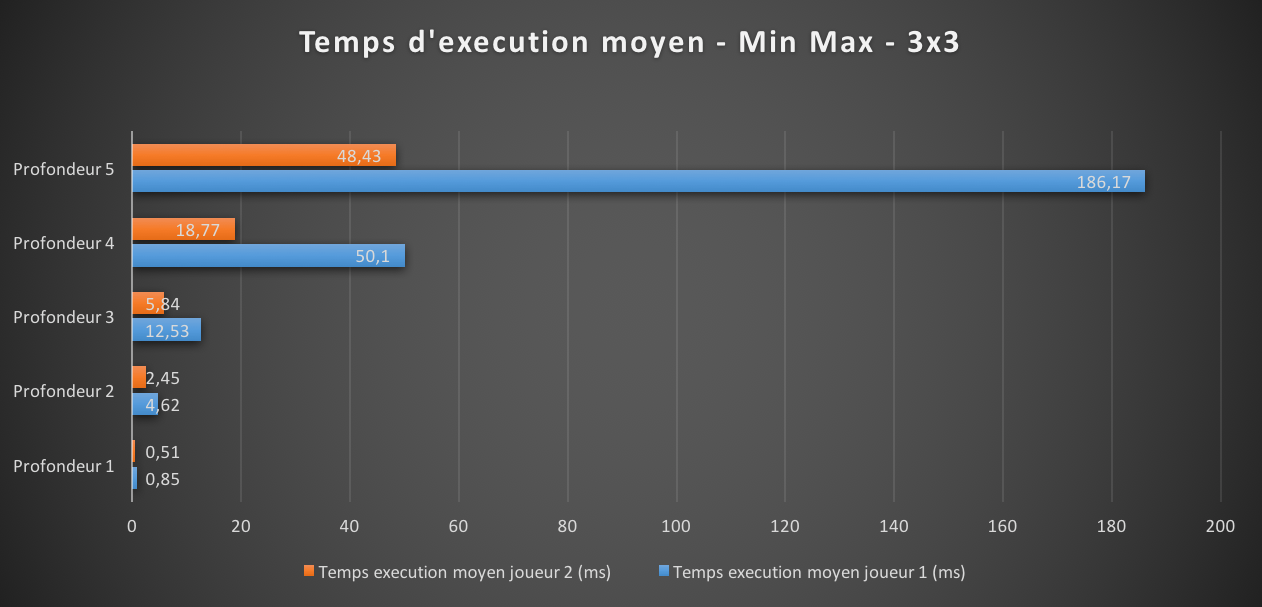
\includegraphics[scale=0.40]{tempsExecutionMinMax3x3.png}
	\end{figure}
     \begin{figure}[!t]
     	    \caption{Temps d'éxecution de l'algorthme min-max avec un plateau 4x4}
     	    \label{TEAMM4x4}
     	    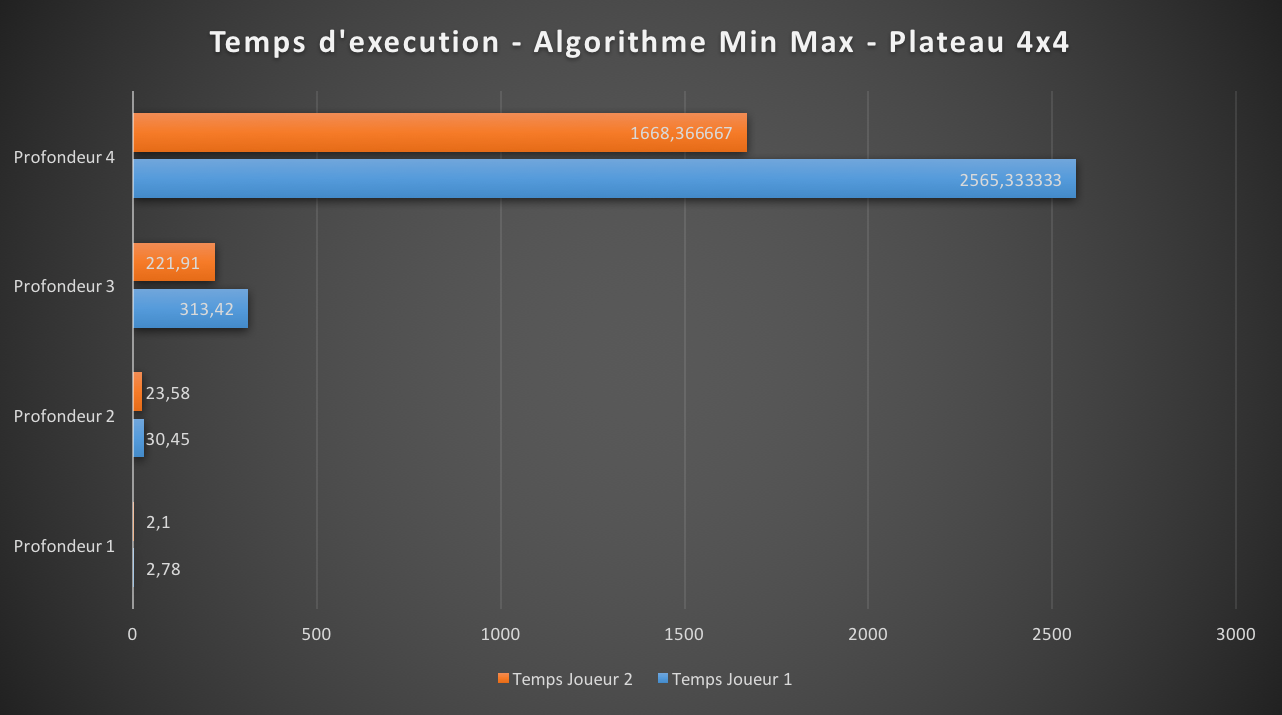
\includegraphics[scale=0.40]{tempsExecutionMinMax4x4.png}
     \end{figure}
	\begin{figure}[!t]
    	    \caption{Temps d'éxecution de l'algorthme min-max avec un plateau 5x5}
    	    \label{TEAMM5x5}
    	    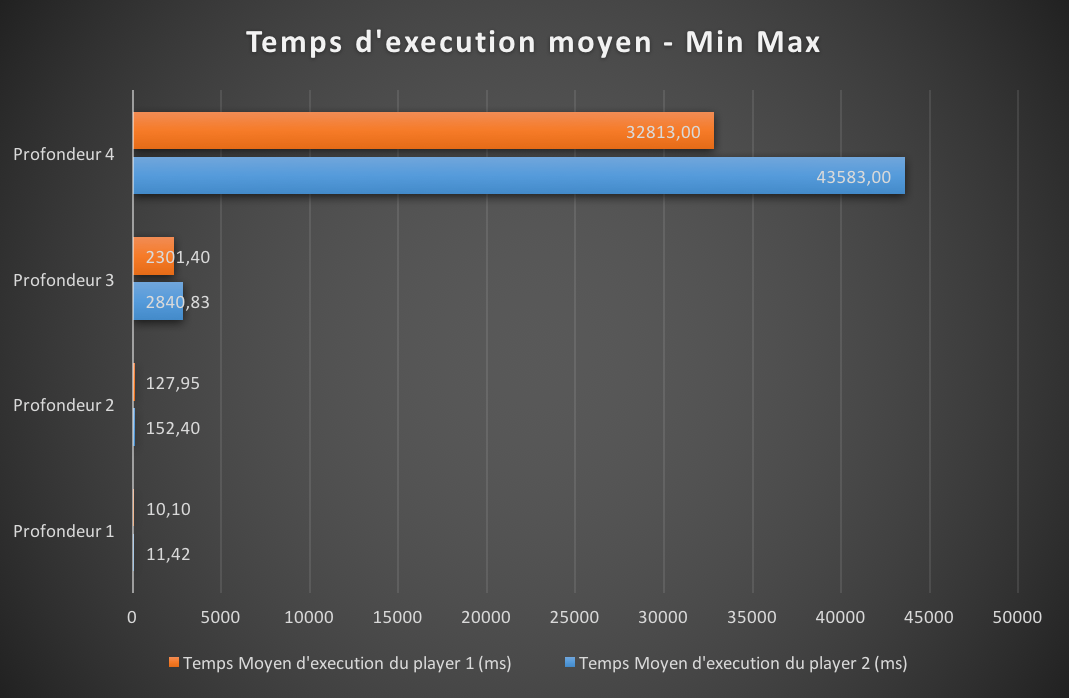
\includegraphics[scale=0.40]{tempsExecutionMinMax5x5.png}
    	\end{figure}


	\subsection{Taux de victoire des differents algorithmes}
	Pour verifier l'efficacité de nos différents algorithmes, nous avons décidé de les faire s'affronter sur un grand nombre de parties. 
	Ainsi nous avons obtenu les graphiques suivants (cf : ) 
	Nous pouvons en conclure que l'algorithme min-max est le plus efficace devant le score-max qui lui-même devance le random. La logique est donc respectée.
	De plus en confrontant les algorithmes les uns contre les autres on peut conclure que le fait d'être le premier joueur au Gomoku est un réel avantage.
	\begin{figure}[!h]
	    \caption{Taux de victoire du random contre le random}
	    \label{TVRandomVSRandom}
	     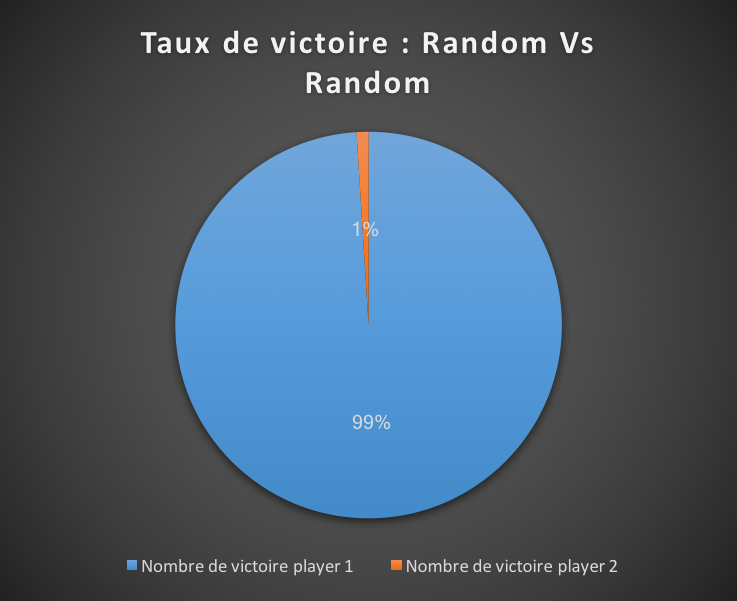
\includegraphics[scale=0.60]{TauxDeVictoireRandomVSRandom.png}
    \end{figure}
    \begin{figure}[!h]
    	    \caption{Taux de victoire du random contre le MaxScore}
    	    \label{TVRandomVMaxScore}
    	     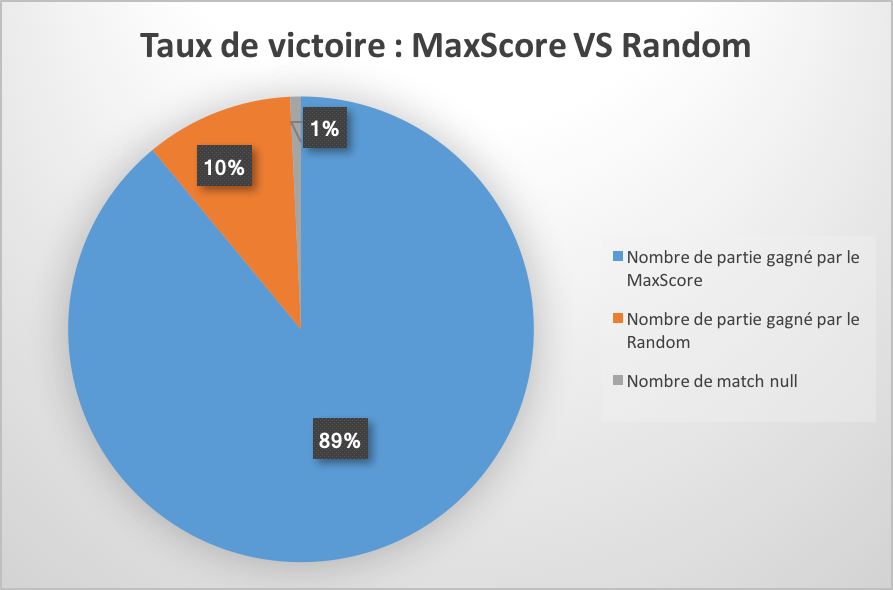
\includegraphics[scale=0.60]{TauxVictoireRandomVsMaxScore.png}
    \end{figure}
    \begin{figure}[!h]
    	    \caption{Taux de victoire du MaxScore contre le MaxScore}
    	    \label{TVMaxScoreVMaxScore}
    	     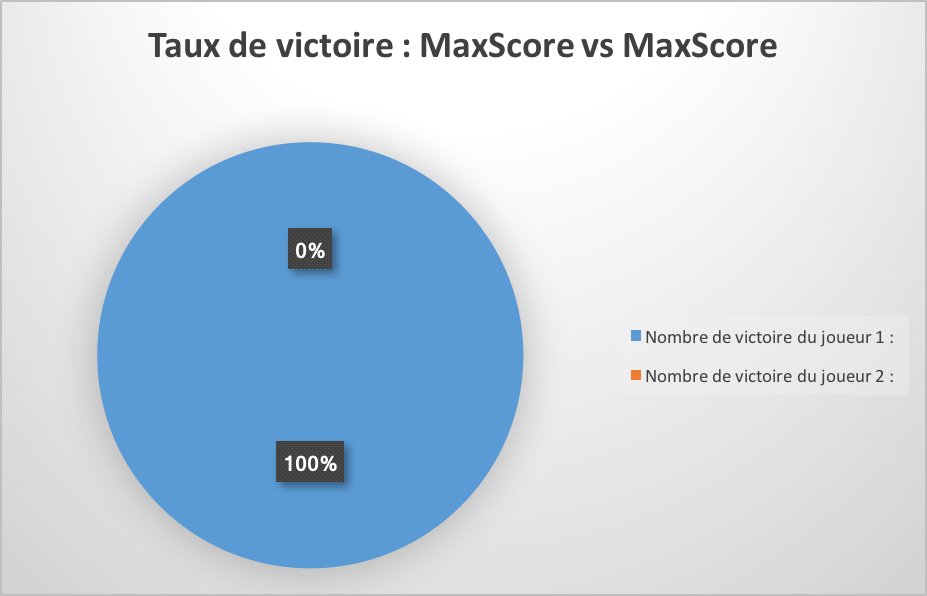
\includegraphics[scale=0.60]{TauxDeVictoireMaxScoreVSMaxScore.png}
    \end{figure}
    \begin{figure}[!h]
    	    \caption{Taux de victoire du MaxScore contre le MinMax}
    	    \label{TVMaxScoreVMaxScore}
    	     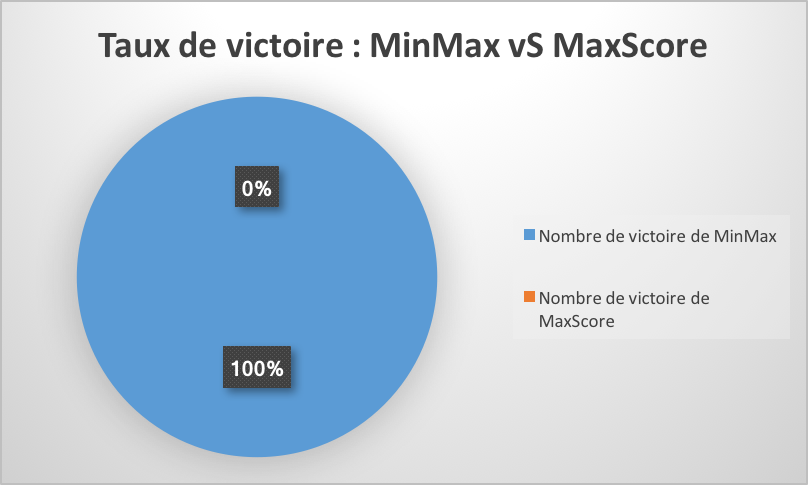
\includegraphics[scale=0.60]{TauxDeVictoireMaxScoreVSMinMax.png}
    \end{figure}
    \begin{figure}[!h]
    	    \caption{Taux de victoire du MinMax contre le MinMax}
    	    \label{TVMaxScoreVMaxScore}
    	     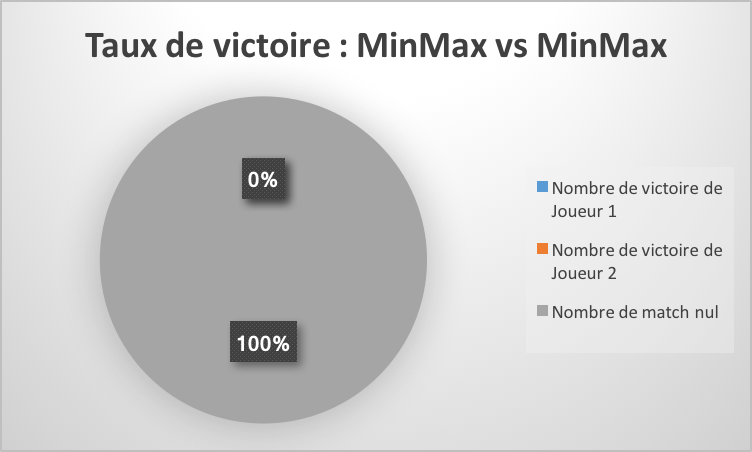
\includegraphics[scale=0.60]{TauxDeVictoireMinMaxVSMinMax}
    \end{figure}
	

\part{Manuel d'utilisation}
	\section{Le développeur}
	% --> Là on peut revenir sur le fait que notre code est bien divisé et que si une personne veut reprendre notre architecture et simplement créer une IA sans se préocuper de la création de l'ensemble du jeux, c'est très simple, il suffit de créer une classe qui extends de IA. 
	% --> Pour lancer des parties qui se jouent seules il suffit de modifier dans Game.... Attention 
	La structure de ce projet à été pensée de telle sorte à permettre à un développeur d'implémenter une nouvelle intelligence artificielle de jeu sans avoir à se préocuper de la partie de gestion des tours, des joueurs. Pour cela il lui suffit de créer une nouvelle classe fille de la classe IA. Il pourra bénéficier de toutes les fonctionnalités de test déjà mises en place.
	
	

	\section{Le joueur}
	% --> Il suffit de lancer le jeux et bim bam boum, il lui suffit de jouer
	% --> A voir si on a le temps de revoir l'interface graphique pour permettre au joueur de choisir son nom, sa couleur, ainsi que l'IA qu'il affrontera
	Pour le joueur il suffit de lancer le jeu à partir de son IDE de programation. 

\part{Rapport d'activité}
% Utilisation de git
% On a beaucoup parlé, utilisation de schémas pour comprendre les algo
% Parler d'une première version avec des clones, et expliquer que le temps etait beaucou beaucoup beaucoup trop long pour être convenable 
Cette partie explique les différentes difficultés rencontrées ainsi que certains choix technologiques de notre part.
\section{git}
Pour réaliser ce projet nous nous sommes servi de gitHub permettant de faire du versionning et ainsi de rendre le travail plus efficace. Il est en efffet possible de voir les différentes évolutions du projet et de revenir en arrière en cas de besoin.
\section{problèmes rencontrés}
\subsection{Algorithme min-max}
 Nous avons du faire un grand nombre de recherches et de tests afin de nous approprier les différents algorithmes et de les implémenter.
Ainsi pour le min-max, nous avions, dans un premier temps, cloné autant de fois qu'il y a de coup à jouer le plateau de jeu. Cela entraine un temps d'exécution considérable car la complexité étant en O(n!), ce temps était inutilement allongé. Par la suite nous avons trouvé une solution pour simuler les différents coups, stocker la valeur et annuler le coup sur un seul plateau de jeu ce qui rendait le temps d'exécution bien plus convenable.(cf tests temps d'exécution).
\subsection{Algorithme alpha-bêta} \label{alphabeta}
Nous avons, suite à l'implémentation de l'algorithme min-max, essayé d'améliorer encore le temps d'exécution sans impacter le taux de victoire grâce à l'algorithme alpha-bêta dont le principe est le même que le min-max mais dont la différence réside dans le fait qu'il limite le nombre de cas testés dans l'arbre de jeu suivant ce principe : si le max du coup suivant est inférieur au min du coup courant alors cette branche ne sera pas explorée. Ainsi seulement les branches menant à une victoire potentielle seront testées et la complexité sera ainsi améliorée.
Les résultats obtenus n'étant pas concluants nous avons décidé d'avorter cette partie du projet. 


\chapter*{Conclusion}
Ce projet en algorithmique a été une bonne introduction à ce qu'est l'intelligence artificielle et les ressorts sur lesquels elle s'appuie.
Nous avons du mettre en place une méthodologie afin de construire, tester et améliorer tout ce que nous faisions au fur et à mesure de l'avancement des choses.
Nous avons apprécié l'autonomie laissée nous obligeant à nous confronter à des problèmes de nature et de complexité diverse afin d'aboutir à quelque chose de fonctionnel
et qui nous convient du point de vue de l'architecture globale.





\end{document}